\begin{longtable} { | c | p{12cm} | c | } 
\hline
	ID 	&	Issues	&		 Es. hours \\\hline
	57	&	Add settings	&	16 hours	\\\hline
	60	&	Settings Intents & \\\hline
\caption{Issue ID 57 and 60}
\label{tab:spr4_addsettings}
\end{longtable}

To manage customer requests to display sequences differently for children, a SettingsActivity was created with two options: The orientation of the screen and how many pictograms to display at a time.

The database had no support for saving settings. This forced us to implement the settings using Android's \ct{sharedPreferences} which is able to store preferences between user sessions \cite{sharedpreferences}. This means that while the preferences are persistent on the tablet they were altered, it is not synchronized with the database at any point.

The settings are saved when the guardian closes the SettingsActivity seen in \ref{fig:profileselector}. They are uniquely saved for each child as the key used to save/fetch the settings includes the ID of the child, which from the database should be guaranteed unique. How the preferences are saved can be seen in \ref{lst:savesettings}. When needed, they can be loaded using Android's \ct{getSharedPreferences}. This is done when calling Sequenceviewer, and the preferences are sent through an \ct{intent} as seen in \ref{lst:loadsettings}.

\begin{figure}[H]
	\centering
	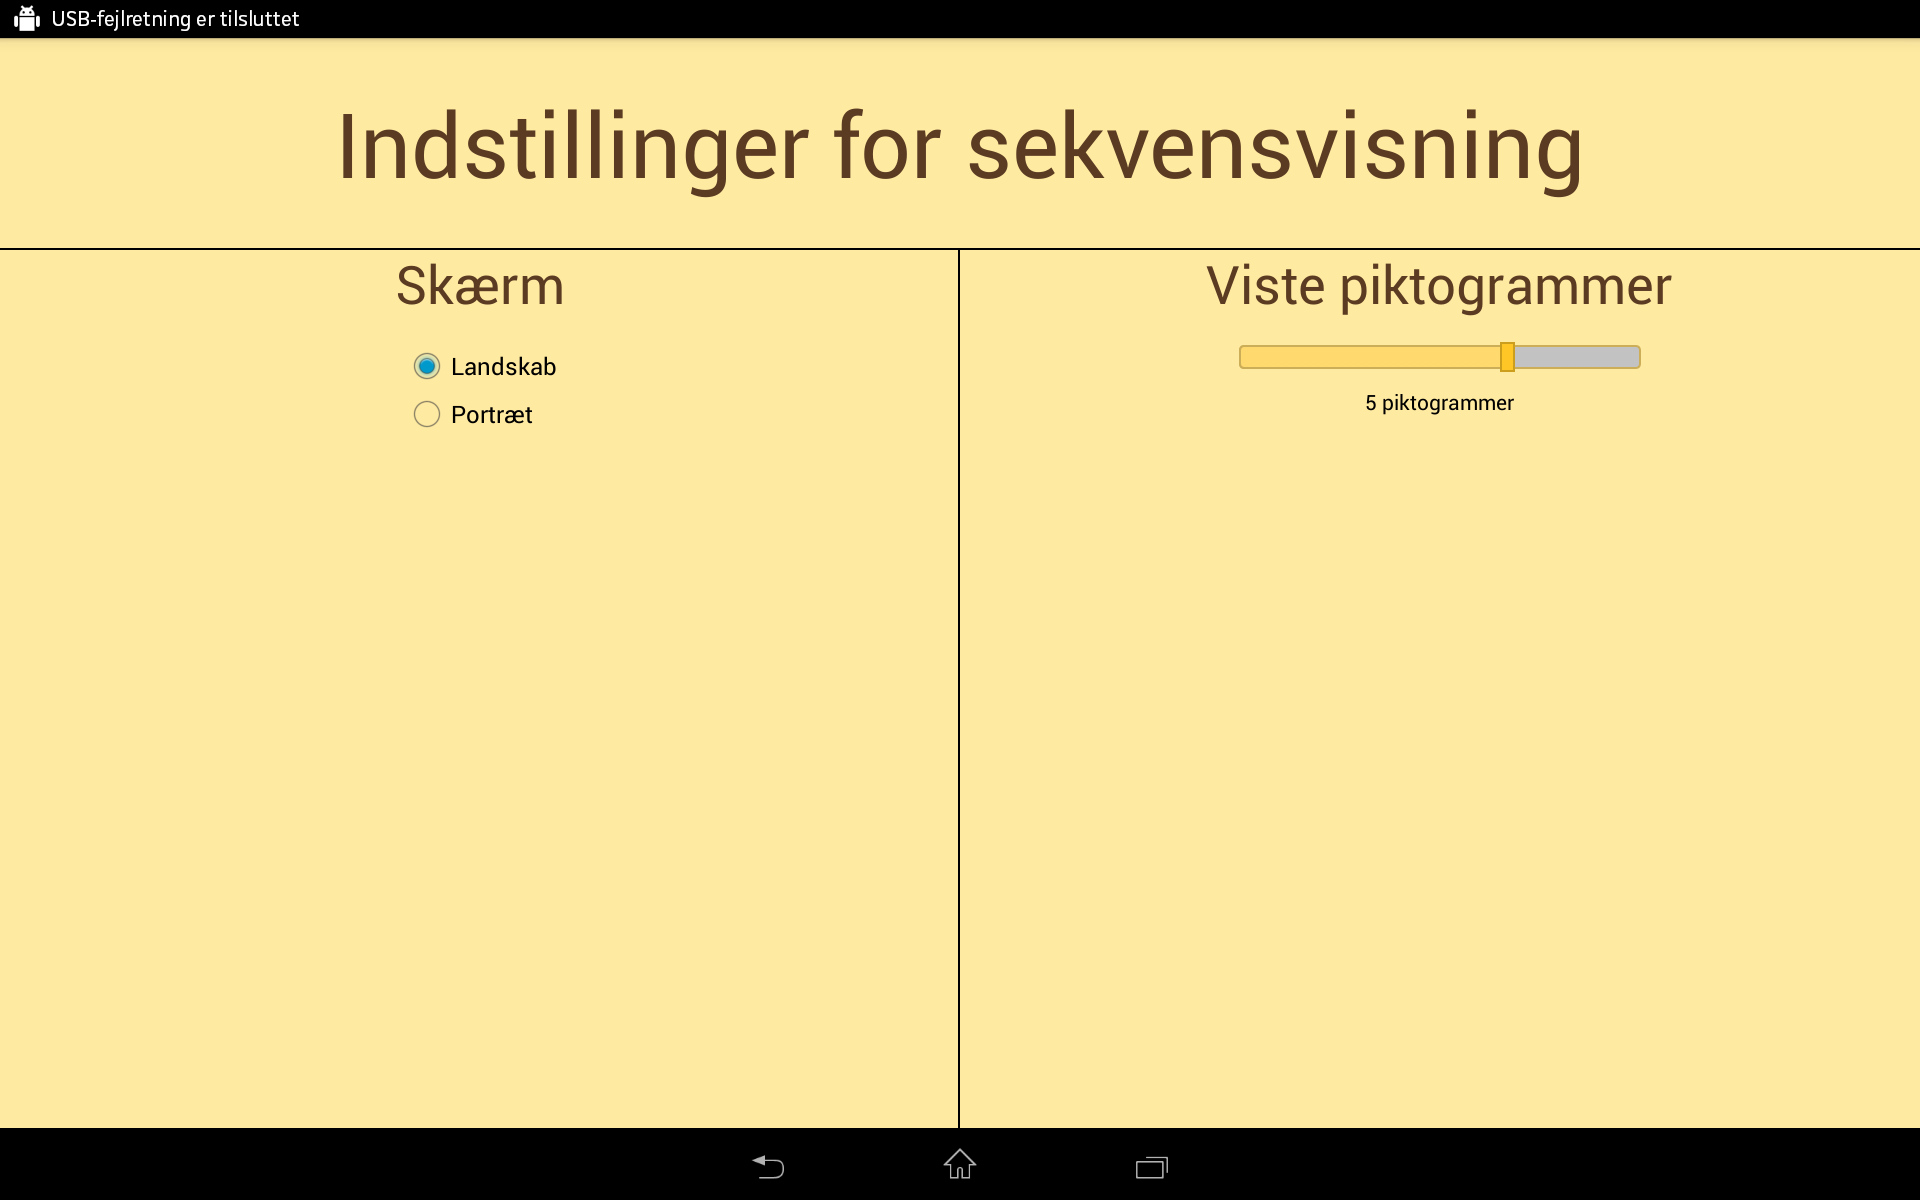
\includegraphics[width=\textwidth]{Pics/Sprint4/settings.png}
	\caption{The SettingsActivity - settings are dependant on the child}
	\label{fig:settingsactivity}
\end{figure}

\begin{lstlisting} [caption={Saving settings for a child}, label={lst:savesettings}]
private void saveSettings() {
    SharedPreferences.Editor editor = settings.edit();
    editor.putInt("pictogramSetting", pictogramSetting);
    editor.putBoolean("landscapeSetting", landscapeSetting);
    editor.commit();
    }
\end{lstlisting}

\begin{lstlisting} [caption={Loading settings and putting them as intents for Sequenceviewer}, label={lst:loadsettings}]
sequenceGrid.setOnItemClickListener(new AdapterView.OnItemClickListener() {
	@Override
	public void onItemClick(AdapterView<?> arg0, View arg1, int arg2, long arg3) {
		((PictogramView) arg1).liftUp();
		assumeMinimize = false;
		
		//Load Preferences
		SharedPreferences settings = getSharedPreferences(SettingsActivity.class.getName() + Integer.toString(selectedChild.getId()), MODE_PRIVATE);
		int pictogramSetting = settings.getInt("pictogramSetting", 5);
		boolean landscapeSetting = settings.getBoolean("landscapeSetting", true);

		//Create Intent with relevant Extras
		Intent intent = new Intent();
		intent.setComponent(new ComponentName("dk.aau.cs.giraf.sequenceviewer", "dk.aau.cs.giraf.sequenceviewer.MainActivity"));
		intent.putExtra("sequenceId", sequenceAdapter.getItem(arg2).getId());
		intent.putExtra("landscapeMode", landscapeSetting);
		intent.putExtra("visiblePictogramCount", pictogramSetting);
		intent.putExtra("callerType", "Zebra");
		startActivityForResult(intent, 2);
		}
	});
}
\end{lstlisting}